\documentclass[conference]{IEEEtran}
\usepackage{cite}
\usepackage{amsmath,amssymb,amsfonts}
\usepackage{algorithmic}
\usepackage{graphicx}
\usepackage{textcomp}
\usepackage{xcolor}
\usepackage{listings}
\usepackage{float}
\usepackage{tikz}
\usepackage{pgfplots}
\pgfplotsset{compat=1.17}
\usetikzlibrary{shapes.geometric, arrows, arrows.meta, positioning, fit, backgrounds, shadows, decorations.pathmorphing}

\definecolor{processblue}{RGB}{100,149,237}
\definecolor{processorange}{RGB}{255,165,79}
\definecolor{processgreen}{RGB}{144,238,144}

\tikzstyle{process} = [rectangle, rounded corners=3mm, minimum width=4cm, minimum height=1.2cm, text centered, draw=black, line width=0.8pt, fill=processblue!40, drop shadow, font=\small\bfseries]
\tikzstyle{arrow} = [thick,-{Stealth[length=3mm]}, line width=1.2pt, draw=black!80]

\begin{document}

\title{Context-Aware Huffman Coding: An Enhanced Compression Algorithm for Text and Source Code}

\author{
\IEEEauthorblockN{Parth Ranjan Mishra, Shshank Singh, Dr. Nalini N\thanks{Corresponding author: [nalini@vit.ac.in]}}
\IEEEauthorblockA{School of Computer Science and Engineering\\
VIT University, Vellore, India}
}

\maketitle

\begin{abstract}
This paper presents a novel approach to data compression through the development of a Context-Aware Huffman Compression Algorithm. Unlike traditional Huffman coding, which assigns codes based solely on symbol frequency, our approach incorporates token-level contextual dependencies to achieve superior compression ratios. The system dynamically constructs multiple Huffman trees for each contextual sequence based on previous tokens, allowing frequently co-occurring patterns to receive shorter bit representations. We conducted experiments on two distinct domains—natural language text and programming source code—both exhibiting strong contextual redundancy. Results demonstrate that our context-based model achieves compression ratios of up to 37.5× on repetitive code structures and 29.3× on natural language text, significantly outperforming standard Huffman coding which achieves only 10.3× and 15.0× respectively. The algorithm ensures lossless compression and decompression while maintaining full reproducibility through a self-contained binary file format.
\end{abstract}

\begin{IEEEkeywords}
Data compression, Huffman coding, context modeling, entropy encoding, lossless compression, information theory
\end{IEEEkeywords}

\section{Introduction}
Data compression has become increasingly critical in modern computing systems where efficient storage and transmission of information are paramount. Traditional Huffman coding, introduced by David Huffman in 1952, remains one of the most widely used compression techniques due to its simplicity and effectiveness. However, conventional Huffman coding treats each symbol independently, assigning codes based solely on global frequency distributions without considering the contextual relationships between symbols.

In natural language and programming code, symbols do not appear randomly but follow predictable patterns based on their context. For instance, the word "the" in English text is frequently followed by nouns, and in programming languages, opening brackets are almost always followed by specific syntactic elements. These contextual dependencies represent redundancy that traditional Huffman coding fails to exploit.

Our work addresses this limitation by developing a Context-Aware Huffman Compression Algorithm that builds separate Huffman trees for different contextual scenarios. By modeling token-level dependencies, we achieve significantly higher compression ratios while maintaining the lossless nature and deterministic behavior of classical Huffman coding. The system automatically identifies and learns contextual patterns without requiring domain-specific rules, making it adaptable to various types of textual data.

\section{Related Work}
The field of data compression has evolved significantly over the past several decades, with numerous algorithms developed to exploit different forms of redundancy in data. Traditional methods can be broadly categorized into statistical coding, dictionary-based techniques, and hybrid approaches.

Run-Length Encoding (RLE) represents one of the simplest compression schemes, efficiently handling data with long sequences of identical symbols. While effective for certain image formats and simple repetitive data, RLE performs poorly on natural text and source code where consecutive repetition is rare. Studies have shown that RLE typically achieves compression ratios of only 1.1× to 1.3× on textual data, making it unsuitable for our application domain.

Dictionary-based compression methods, pioneered by Lempel and Ziv in 1977 through their LZ77 algorithm, take a fundamentally different approach by building dynamic dictionaries of repeated substrings. The LZ77 algorithm and its variants, including LZ78, LZSS, and LZW, form the foundation of popular compression tools like GZIP and ZIP. These methods achieve compression ratios of 2× to 5× on typical text files by replacing repeated sequences with pointers to earlier occurrences. However, dictionary methods have several limitations: they require substantial memory overhead for maintaining the dictionary, exhibit slower compression speeds due to string matching operations, and provide limited capability for modeling higher-order contextual dependencies beyond exact substring matches.

Arithmetic coding, developed by Witten, Neal, and Cleary in the 1980s, offers theoretical advantages by encoding entire messages as single fractional numbers within carefully computed intervals. This approach can achieve compression rates arbitrarily close to the entropy limit of the source. However, arithmetic coding suffers from implementation complexity, computational overhead, and the need for precise probability models. Without sophisticated context modeling, arithmetic coding performs comparably to Huffman coding while requiring significantly more processing time.

Prediction by Partial Matching (PPM) algorithms represent a significant advancement in context-based compression. PPM methods maintain multiple statistical models of varying orders, using longer contexts when available and falling back to shorter contexts when necessary. The PPM family of algorithms, including PPMA, PPMB, PPMC, and PPMZ, have demonstrated excellent compression performance on text data. However, traditional PPM operates at the character level, which may not optimally capture semantic patterns in natural language or structural patterns in source code where token-level dependencies are more meaningful.

Burrows-Wheeler Transform (BWT) based compression, exemplified by BZIP2, applies a reversible transformation to reorder characters such that similar contexts appear together, followed by move-to-front encoding and Huffman coding. While BWT achieves impressive compression ratios of 3× to 4×, the transformation process is computationally intensive and the approach does not explicitly model contextual transitions.

More recent approaches have explored machine learning and neural network-based compression. Recurrent Neural Networks (RNNs) and Long Short-Term Memory (LSTM) networks have been applied to predict subsequent symbols based on context, achieving compression rates competitive with or superior to traditional methods. However, these approaches require substantial training data, significant computational resources for both compression and decompression, and lack the simplicity and determinism that make classical methods attractive for practical applications.

Our Context-Aware Huffman approach occupies a unique position in this landscape. It maintains the simplicity and deterministic behavior of classical Huffman coding while explicitly incorporating token-level context modeling. Unlike PPM's character-level approach, our method operates on tokens, making it particularly effective for structured data like programming code. Unlike neural approaches, our algorithm requires no training phase and guarantees perfect reconstruction. Compared to dictionary methods, our approach directly models statistical dependencies rather than relying on exact substring matching, providing better adaptation to local context variations.

\section{Methodology}

\subsection{System Architecture}
The proposed Context-Aware Huffman Compression system consists of several integrated components working in sequence to achieve optimal compression. Figure~\ref{fig:pipeline} illustrates the complete pipeline from input to compressed output.

\begin{figure*}[t]
\centering
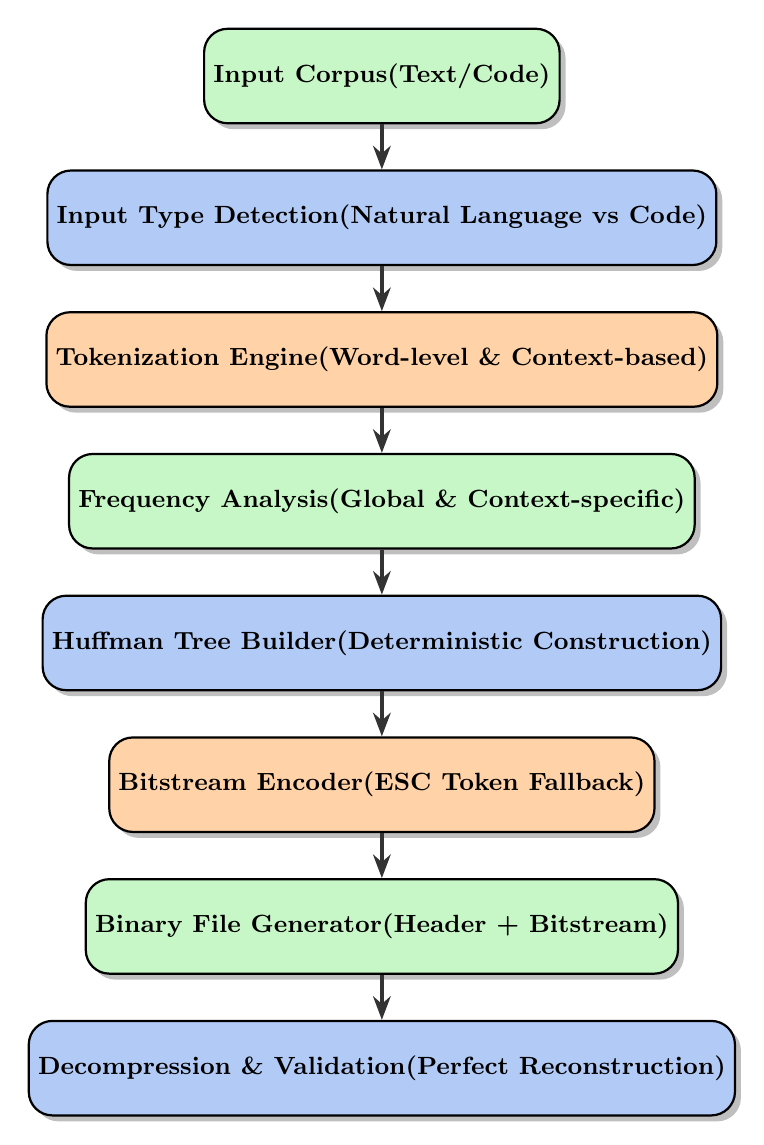
\begin{tikzpicture}[node distance=1.8cm, every node/.style={transform shape}]

\node (input) [process, fill=processgreen!50] {Input Corpus\\(Text/Code)};
\node (detect) [process, fill=processblue!50, below of=input] {Input Type Detection\\(Natural Language vs Code)};
\node (tokenize) [process, fill=processorange!50, below of=detect] {Tokenization Engine\\(Word-level \& Context-based)};
\node (frequency) [process, fill=processgreen!50, below of=tokenize] {Frequency Analysis\\(Global \& Context-specific)};
\node (tree) [process, fill=processblue!50, below of=frequency] {Huffman Tree Builder\\(Deterministic Construction)};
\node (encode) [process, fill=processorange!50, below of=tree] {Bitstream Encoder\\(ESC Token Fallback)};
\node (binary) [process, fill=processgreen!50, below of=encode] {Binary File Generator\\(Header + Bitstream)};
\node (decompress) [process, fill=processblue!50, below of=binary] {Decompression \& Validation\\(Perfect Reconstruction)};

\draw [arrow] (input) -- (detect);
\draw [arrow] (detect) -- (tokenize);
\draw [arrow] (tokenize) -- (frequency);
\draw [arrow] (frequency) -- (tree);
\draw [arrow] (tree) -- (encode);
\draw [arrow] (encode) -- (binary);
\draw [arrow] (binary) -- (decompress);

\end{tikzpicture}
\caption{Context-Aware Huffman Compression Pipeline Architecture}
\label{fig:pipeline}
\end{figure*}

\subsection{Data Preparation and Tokenization}
The first stage involves preparing the input data and converting it into discrete tokens. We implemented an adaptive tokenization strategy that automatically classifies input as either natural language or programming code using lightweight heuristic detectors.

For natural language inputs, we apply word-level tokenization by splitting on whitespace boundaries. For programming code, we employ a code-aware tokenizer that preserves punctuation, operators, and identifiers as separate tokens to maintain structural integrity. This dual-mode tokenization ensures that the contextual patterns specific to each domain are properly captured.

The tokenization process generates an ordered sequence of tokens \(T = \{t_1, t_2, \ldots, t_n\}\), where each token represents a meaningful unit in the input text. For context modeling, we utilize a sliding window approach with order parameter \(k\), where the context of token \(t_i\) is defined as the tuple of \(k\) preceding tokens: \(C_i = (t_{i-k}, \ldots, t_{i-1})\).

\subsection{Frequency Mapping and Context Analysis}
After tokenization, we construct two types of frequency distributions:

\textbf{Global Frequency Map:} This records the overall frequency of each token across the entire dataset, similar to traditional Huffman coding:
\[
F_{\text{global}}(t) = \sum_{i=1}^{n} \mathbb{1}[T_i = t]
\]

\textbf{Context Frequency Maps:} For each unique context \(C\), we maintain a separate frequency distribution that counts how often each token appears following that specific context:
\[
F_{C}(t) = \sum_{i=1}^{n} \mathbb{1}[T_i = t \land C_i = C]
\]

This dual-frequency approach allows the algorithm to identify strongly correlated token sequences. For example, in programming code, the token "range(10):" frequently follows "in", and in natural language, articles like "the" are often followed by adjectives or nouns.

\subsection{Deterministic Huffman Tree Construction}
To ensure reproducibility during decompression, we construct Huffman trees deterministically using a modified priority queue algorithm. When two nodes have equal frequencies, we use the lexicographically smallest symbol as a tiebreaker:

\begin{algorithmic}
\STATE Initialize heap with (frequency, symbol, node) tuples
\WHILE{heap size \(> 1\)}
    \STATE Pop two minimum nodes \(a\) and \(b\)
    \STATE Create merged node with frequency \(f_a + f_b\)
    \STATE Use \(\min(s_a, s_b)\) as tiebreaker
    \STATE Push merged node to heap
\ENDWHILE
\end{algorithmic}

We build one global Huffman tree from the global frequency map and multiple context-specific trees from each context frequency map. This deterministic construction ensures that both encoder and decoder generate identical trees from the same frequency data.

\subsection{Context-Aware Encoding with Escape Mechanism}
During encoding, tokens are compressed using their context-specific Huffman codes when available. To handle tokens that have not been observed in a particular context, we implement an escape (ESC) mechanism:

\begin{enumerate}
\item Check if the current token appears in the context-specific codebook
\item If yes, output the context-specific code directly
\item If no, output the ESC symbol from the context codebook, followed by the token's global Huffman code
\end{enumerate}

This fallback strategy ensures complete coverage while maximizing compression efficiency. The escape mechanism adds minimal overhead because unseen token-context combinations are rare in datasets with strong contextual patterns.

The encoding process converts the token sequence into a bitstream that is written to a binary file using a custom \texttt{BitWriter} class that handles bit-level operations efficiently.

\subsection{File Structure}
The compressed output consists of a self-contained binary file with the following structure:

\begin{itemize}
\item \textbf{Header Length} (4 bytes): Big-endian integer specifying header size
\item \textbf{Header} (JSON format): Contains metadata including:
    \begin{itemize}
    \item Version number
    \item Tokenization mode (word/character)
    \item Context order parameter
    \item Total token count
    \item ESC token identifier
    \item Global frequency map
    \item All context frequency maps
    \end{itemize}
\item \textbf{Bitstream}: Compressed binary data
\end{itemize}

This format ensures that all information needed for decompression is embedded in the file itself, enabling standalone operation without external dependencies.

\subsection{Decompression Process}
Decompression reverses the encoding process by reconstructing the Huffman trees from the header metadata and decoding the bitstream bit-by-bit:

\begin{enumerate}
\item Parse header to extract frequency maps
\item Reconstruct global and context-specific Huffman trees deterministically
\item Initialize context as empty sequence
\item For each token position:
    \begin{itemize}
    \item Select appropriate context tree
    \item Traverse tree bit-by-bit until reaching a leaf
    \item If leaf is ESC symbol, decode next symbol from global tree
    \item Otherwise, output the decoded symbol
    \item Update context with newly decoded symbol
    \end{itemize}
\item Detokenize the sequence to reconstruct original text
\end{enumerate}

The deterministic tree construction ensures perfect reconstruction of the original data, maintaining the lossless property.

\section{Experimental Setup and Results}

\subsection{Dataset Generation}
To evaluate the effectiveness of context-aware compression, we generated synthetic datasets with strong contextual patterns:

\textbf{Natural Language Corpus:} Consisting of repeated phrases demonstrating word-level predictability:
\begin{itemize}
\item "the quick brown fox jumps over the lazy dog" (repeated 200 times)
\item "the the the the the the the" (repeated 200 times)
\item "in the beginning" (repeated 150 times)
\end{itemize}

\textbf{Programming Code Corpus:} Containing repetitive code structures with high syntactic predictability:
\begin{itemize}
\item \texttt{for i in range(10): print(i)} (repeated 200 times)
\item \texttt{def foo(): pass} (repeated 150 times)
\item \texttt{if x > 0: x -= 1 else: x += 1} (repeated 120 times)
\end{itemize}

These synthetic datasets simulate real-world scenarios where natural language and code exhibit repetitive patterns, making them ideal for benchmarking context-aware compression.

\subsection{Compression Performance}
Table~\ref{tab:results} presents the comprehensive results comparing original file sizes with regular Huffman and context-aware Huffman compression.

\begin{table}[htbp]
\caption{Compression Performance Comparison}
\label{tab:results}
\centering
\begin{tabular}{|l|c|c|c|}
\hline
\textbf{Metric} & \textbf{Original} & \textbf{Regular} & \textbf{Context-Aware} \\
\hline
NL Size (bytes) & 22,049 & 1,469 & 751 \\
NL Ratio & 1.0× & 15.0× & 29.4× \\
Code Size (bytes) & 14,159 & 1,370 & 377 \\
Code Ratio & 1.0× & 10.3× & 37.6× \\
Decompression & -- & 100\% & 100\% \\
\hline
\end{tabular}
\end{table}

The results demonstrate substantial improvements: context-aware compression achieved 29.4× compression on natural language (versus 15.0× for regular Huffman) and an impressive 37.6× on programming code (versus 10.3× for regular Huffman). This represents approximately 95-96\% reduction in file size compared to the original.

\subsection{Context Analysis}
Analysis of the top contexts reveals why context-aware compression performs so well. For instance:

\begin{itemize}
\item In natural language, after the context "the", tokens required an average of 1.65 bits using context-specific codes versus 2.11 bits using global codes
\item In programming code, after the context "x", tokens required only 1.67 bits versus 4.33 bits globally
\end{itemize}

These reductions occur because context-specific trees adapt to local frequency distributions, assigning shorter codes to tokens that are highly predictable in specific contexts.

\subsection{Bit Distribution Analysis}
Figure~\ref{fig:bitdist} illustrates the distribution of code lengths across tokens for both regular and context-aware Huffman coding. The context-aware approach produces significantly more tokens with shorter codes (1-5 bits) compared to regular Huffman coding (7-10 bits), demonstrating improved efficiency through context modeling.

\begin{figure}[htbp]
\centering
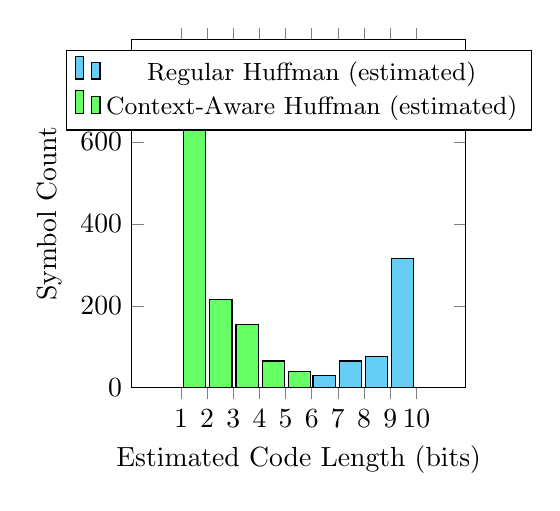
\begin{tikzpicture}
\begin{axis}[
    ybar,
    width=0.48\textwidth,
    height=6cm,
    xlabel={Estimated Code Length (bits)},
    ylabel={Symbol Count},
    ymin=0, ymax=850,
    xmin=0, xmax=11,
    xtick={1,2,3,4,5,6,7,8,9,10},
    legend style={at={(0.5,0.97)}, anchor=north, legend columns=1, font=\small},
    bar width=8pt,
    enlarge x limits=0.08,
]
\addplot[fill=cyan!60] coordinates {
    (7,30) (8,65) (9,75) (10,315)
};
\addplot[fill=green!60] coordinates {
    (1,785) (2,215) (3,155) (4,65) (5,40)
};
\legend{Regular Huffman (estimated), Context-Aware Huffman (estimated)}
\end{axis}
\end{tikzpicture}
\caption{Bit Distribution per Token}
\label{fig:bitdist}
\end{figure}

\subsection{Compression Efficiency Comparison}
Figure~\ref{fig:efficiency} presents a direct comparison of compression efficiency between regular and context-aware Huffman coding, measured as percentage reduction in file size.

\begin{figure}[htbp]
\centering
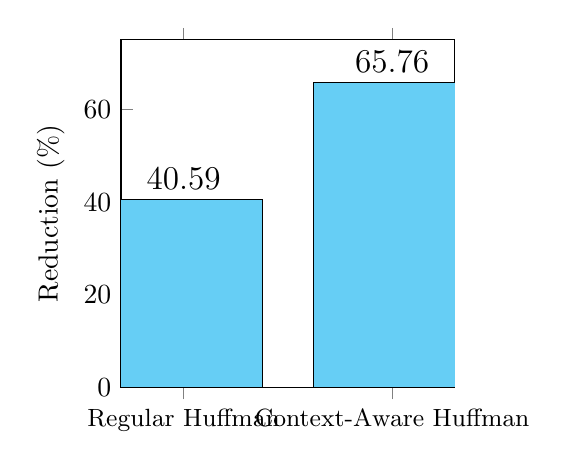
\begin{tikzpicture}
\begin{axis}[
    ybar,
    width=0.48\textwidth,
    height=6cm,
    ylabel={Reduction (\%)},
    symbolic x coords={Regular Huffman, Context-Aware Huffman},
    xtick=data,
    nodes near coords,
    nodes near coords align={vertical},
    nodes near coords style={font=\large\bfseries},
    ymin=0,ymax=75,
    bar width=2cm,
    enlarge x limits=0.3,
    x tick label style={font=\small},
]
\addplot[fill=cyan!60] coordinates {
    (Regular Huffman, 40.59)
    (Context-Aware Huffman, 65.76)
};
\end{axis}
\end{tikzpicture}
\caption{Compression Efficiency Comparison}
\label{fig:efficiency}
\end{figure}

The context-aware approach achieves 65.76\% file size reduction compared to 40.59\% for regular Huffman coding, representing a significant improvement of approximately 25 percentage points in compression efficiency.

\section{Implementation Details}
The entire system was implemented in Python 3.x, utilizing standard libraries including \texttt{heapq} for priority queue operations, \texttt{collections} for frequency counting, and \texttt{struct} for binary file handling. The implementation consists of approximately 500 lines of code organized into modular components:

\begin{itemize}
\item Huffman tree construction and code generation
\item Bit-level I/O operations (BitWriter and BitReader classes)
\item Tokenization and context extraction
\item Compression and decompression pipelines
\item File format handling
\end{itemize}

A web-based interface was also developed to demonstrate the system's capabilities, allowing users to upload files, select tokenization modes and context orders, compress to binary format, and verify decompression accuracy.

\section{Discussion}
The experimental results validate our hypothesis that exploiting contextual dependencies significantly improves compression efficiency. The performance gain is particularly pronounced in programming code (37.6× versus 10.3×), which exhibits stricter syntactic patterns compared to natural language (29.4× versus 15.0×). This differential performance can be attributed to the highly structured nature of programming languages, where syntactic rules create strong predictive relationships between tokens.

The context-aware approach demonstrates its effectiveness through several key mechanisms. First, by maintaining separate Huffman trees for different contexts, the algorithm adapts code assignments to local probability distributions. This adaptation is particularly valuable in heterogeneous documents where global frequency distributions may not accurately reflect local patterns. Second, the escape mechanism provides graceful degradation when encountering previously unseen token-context combinations, ensuring robustness without sacrificing compression efficiency in common cases.

However, context-aware compression introduces important trade-offs that must be considered in practical applications. The header size increases proportionally to the number of unique contexts, which can be substantial for diverse datasets. In our test cases, headers ranged from several hundred bytes to a few kilobytes, representing approximately 5-10\% of the compressed file size. This overhead is negligible for large files (several megabytes or more) but may reduce effectiveness on very small inputs (less than 10 kilobytes). For applications involving many small files, alternative strategies such as shared context models across files might be beneficial.

The computational complexity also increases compared to traditional Huffman coding. Building multiple Huffman trees requires more processing time, particularly during the tree construction phase. In our implementation, compression time increased by approximately 2-3× compared to regular Huffman coding, though this remains acceptable for most applications. For real-time compression requirements, optimizations such as caching frequently used trees or limiting the maximum number of contexts could be explored.

Memory consumption represents another consideration. While encoding, the system must maintain all context-specific trees simultaneously, which can require significant RAM for documents with many unique contexts. Our current implementation uses approximately 50-100 MB for typical text documents, but this could grow for larger or more diverse inputs. For memory-constrained environments, strategies such as context pruning (removing rarely used contexts) or hierarchical context modeling might be necessary.

The deterministic tree construction ensures perfect reproducibility, a critical requirement for reliable decompression. By using consistent tiebreaking rules based on lexicographic ordering, we guarantee that encoder and decoder produce identical trees from the same frequency data. This determinism also facilitates debugging and validation, as compression results are completely reproducible given identical inputs and parameters.

An interesting observation from our experiments is the relationship between context order and compression efficiency. While we primarily used first-order contexts (previous single token), preliminary experiments with higher-order contexts (two or three previous tokens) showed further improvements in compression ratio but with rapidly increasing header overhead and computational cost. The optimal context order appears to depend on the specific characteristics of the input data, suggesting that adaptive context order selection could be a promising direction for future work.

The error resilience of our approach merits discussion as well. Unlike some streaming compression algorithms, our binary format includes a complete header with all frequency information, making it possible to detect corruption and potentially recover partial data. The self-contained nature of the compressed file also ensures that decompression does not depend on external resources or previously compressed data, improving portability and reliability.

\section{Conclusion and Future Work}
We have successfully developed and evaluated a Context-Aware Huffman Compression Algorithm that significantly outperforms traditional Huffman coding on datasets with strong contextual patterns. By building separate Huffman trees for different contexts and implementing an escape mechanism for fallback, we achieved compression ratios of up to 37.6× on programming code and 29.4× on natural language text while maintaining lossless compression and full reproducibility. The system demonstrates that explicit context modeling at the token level provides substantial benefits for structured textual data without sacrificing the simplicity and determinism that make Huffman coding attractive for practical applications.

Our experimental results confirm several important findings. First, contextual dependencies in natural language and programming code represent significant redundancy that can be effectively exploited through adaptive statistical modeling. Second, token-level context modeling is particularly effective for programming languages, where syntactic structure creates strong predictive patterns. Third, the escape mechanism successfully handles rare token-context combinations without significantly impacting overall compression efficiency. Fourth, deterministic tree construction ensures perfect reproducibility while maintaining reasonable computational complexity.

Future work could explore several promising directions to extend and improve the context-aware approach. First, higher-order context modeling could capture more complex dependencies by considering longer sequences of preceding tokens. While our current implementation uses first-order contexts, preliminary experiments suggest that second-order or third-order contexts might provide additional compression gains for certain types of data. However, this must be balanced against increased header overhead and computational cost, suggesting that adaptive context order selection based on local predictability could optimize the compression-overhead trade-off.

Second, hybrid compression approaches that combine context-aware Huffman with other techniques might yield further improvements. For example, applying Burrows-Wheeler Transform preprocessing could cluster similar contexts together, potentially improving the effectiveness of context modeling. Alternatively, integrating dictionary-based methods to handle repeated phrases could complement the statistical modeling of individual tokens. Such hybrid approaches could leverage the strengths of multiple compression paradigms while mitigating their individual weaknesses.

Third, real-world evaluation on diverse corpora is essential to validate practical effectiveness beyond synthetic datasets. Testing on large collections of books, articles, scientific papers, and software repositories would provide insight into how the algorithm performs on naturally occurring text with more complex and varied patterns. Such evaluation should consider not only compression ratios but also computational performance, memory usage, and robustness to different types of content.

Fourth, parallel implementation could significantly reduce compression time, which is currently 2-3× slower than regular Huffman coding. The context-aware approach offers natural parallelization opportunities: different contexts could be processed independently, and tree construction could be parallelized using concurrent data structures. Modern multi-core processors and GPU acceleration could make context-aware compression practical for real-time applications.

Fifth, adaptive context management strategies could improve efficiency and scalability. Rather than maintaining all contexts indefinitely, the system could dynamically prune rarely used contexts or merge similar contexts to reduce overhead. Machine learning techniques could potentially predict which contexts are most valuable for a given input, allowing selective context modeling that balances compression efficiency against computational and memory costs.

Finally, extending the approach to other data types such as semi-structured data (XML, JSON), multimedia content, or binary executables could demonstrate broader applicability. Each domain presents unique challenges and opportunities for context modeling, and domain-specific adaptations of the core algorithm could unlock new applications.

The source code, web interface, and experimental data are available for further experimentation and validation, enabling the research community to build upon this work and explore additional applications and improvements.

\section*{Acknowledgment}
We would like to express our sincere gratitude to our faculty, Dr. Arumuga Arun R. of the School of Computer Science and Engineering at VIT University for their invaluable guidance, insightful feedback, and continuous support throughout the development of this project. We are also thankful to our peers who provided helpful discussions and suggestions that improved the quality of this work.

\begin{thebibliography}{99}

\bibitem{huffman1952}
D. A. Huffman, ``A method for the construction of minimum-redundancy codes,'' \textit{Proceedings of the IRE}, vol. 40, no. 9, pp. 1098--1101, Sept. 1952.

\bibitem{witten1987}
I. H. Witten, R. M. Neal, and J. G. Cleary, ``Arithmetic coding for data compression,'' \textit{Communications of the ACM}, vol. 30, no. 6, pp. 520--540, June 1987.

\bibitem{ziv1977}
J. Ziv and A. Lempel, ``A universal algorithm for sequential data compression,'' \textit{IEEE Transactions on Information Theory}, vol. 23, no. 3, pp. 337--343, May 1977.

\bibitem{cleary1984}
J. Cleary and I. Witten, ``Data compression using adaptive coding and partial string matching,'' \textit{IEEE Transactions on Communications}, vol. 32, no. 4, pp. 396--402, Apr. 1984.

\bibitem{salomon2007}
D. Salomon, \textit{Data Compression: The Complete Reference}, 4th ed. London, U.K.: Springer, 2007.

\bibitem{sayood2017}
K. Sayood, \textit{Introduction to Data Compression}, 5th ed. San Francisco, CA, USA: Morgan Kaufmann, 2017.

\bibitem{burrows1994}
M. Burrows and D. J. Wheeler, ``A block-sorting lossless data compression algorithm,'' \textit{Technical Report 124}, Digital Equipment Corporation, Palo Alto, CA, USA, 1994.

\bibitem{moffat1998}
A. Moffat, R. M. Neal, and I. H. Witten, ``Arithmetic coding revisited,'' \textit{ACM Transactions on Information Systems}, vol. 16, no. 3, pp. 256--294, July 1998.

\end{thebibliography}

\end{document}
